% Chapter 2

\chapter{Content-control software and providers} % Main chapter title

\label{Chapter2} % For referencing the chapter elsewhere, use \ref{Chapter1}

Content control policies can be implemented at different levels. Some ISPs offer parental control options and even parental control software, other content control systems are integrated with the operating system, such as MacOS, which offers parental controls for some applications (Mail, Finder, iChat, Safari). The two major forms of content filtering technology are application gateway and packet inspection. The application gateway is called web-proxy for HTTP access and works by inspecting the request and the returned page using some rules and deciding if it should return the response. The packet inspection technique does not interfere with the connection, but inspect the data as it goes past and may decide at a later point to disconnect the client, by inject a TCP-Reset or similar faked packet. A combination of these two techniques is very popular because it allows more detailed filtering and can significantly reduce the cost of the system.

We will present next some parental control application and their features, on which we will try to build our system by taking a more self-regulatory approach.

\section{Net Nanny}

Net Nanny provides a content-control software as a way to monitor and control children's computer activity. The main features include blocking and filtering Internet content, place time limits on use and block PC games. Websites are blocked by content rather than URL, preventing children from accessing blocked websites through proxy websites. It is available on desktop platforms, Windows and Mac, and also on mobile platforms, Android and iOS, but the features and usability is not consistent on all platform, with some key features lacking on the mobile. It uses a dynamic filter that scans and analyses each web site to determine if it is appropriate for a child, based on a unique customization done by the parent. All the initial configuration is done online and it enforces the rules via a local client on each device it is installed. For each client, you can select from 4 profiles: Child, Pre-Teen, Teen and Adult, which can be further customized. \parencite{netNannyFeatures}

\subsection{Content Filtering}

Content filtering is the most used feature in all parental control systems and Net Nanny filters by analyzing the content for each web page in real time. Each site is matched against 17 objectionable categories, and each child profile have different level of blocking. Some categories are not completely blocked for some profiles, but the parents get a notification when the child visit sites in these categories. Parents can also create custom rules, to temporary allow access for some devices, and whitelists and blacklists for each child, to always allow or block certain websites. We follow the same approach by creating two classes of users for domain filtering and use a custom blocking mechanism to block certain domains for children, while allowing them for parent users. \parencite{netNannyTomsGuide}

\begin{figure}[th]
\centering
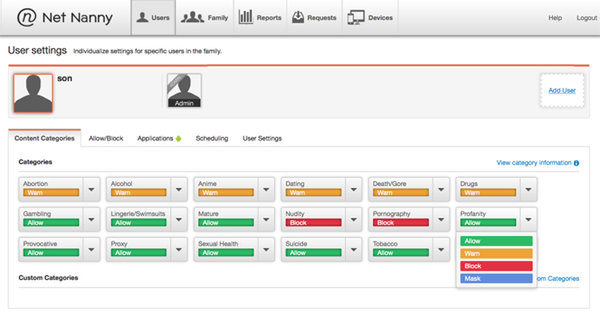
\includegraphics[width=1\textwidth]{Figures/netnanny}
\decoRule
\caption{You can block content categories with Net Nanny's Web filtering tools.}
\label{fig:circle}
\end{figure}

\subsection{Internet Time Scheduling}

Children's internet use can be controlled in two ways using Net Nanny, by creating weekly schedules in half-hour increments, and you can also create weekly allowance duration in one-hour increments. This system does not depend on the system clock, so it cannot be bypassed. But it would be more useful to have more granularity when setting time limits, that's why we support 15-minute increments allowance periods for each day.

\subsection{Email notifications}

Net Nanny have two types of email notifications enabled. The first type of notification is sent when a child request a blocking exception for a specific domain, and the other one is in the form of a weekly summary. You can configure to get notification for multiple types of events, when a child hits a blocked site, continues after a warning or request a change in the blocking status. It would be more useful to have multiple options of getting notified about certain events occurring in the system, that's why we introduced mobile notifications into our system.

\subsection{Detailed Reporting}

Net Nanny offers an online console where you can view all the activity reports. You can view the activity by day, week and month, but not older than 30 days. It shows the blocked content in a pie chart, with some more information on mouse over. The report goes as deep as to show the page title, the time stamp and the user for each URL visited on a specific device. we do not include any type of reporting, because we thing that it would be a privacy issue for the child, since we try to implement a self-regulation system. All the discussion should be done in the family and the child should be warned about visiting certain domains, but not by checking every move he makes online. That's why we don't include any location related features, and Net Nanny does not support location either, but some other parental control systems do.

\subsection{Mobile Support}

The mobile support for Net Nanny is similar to the desktop experience, with some limitations. For the system to work, all the browsing should be done through the proprietary browser offered. On the iPhone the features are even more limited, because it does not interact with other apps and services at all. Since we started developing for mobile first and we try to keep the application features decoupled from the client device and system, we should not suffer of these limitations and we provide a seamless experience on both mobile platform, Android and iOS. \parencite{netNannyPCMag}

\section{Qustodio}

Qustodio is a parental control tool that runs on any device, from PC to Android and iOS and even on Kindle devices. It has a lot of features, from web content filtering, app blocking and detailed activity logs. The configuration and monitoring is handled either through an online dashboard or a mobile control application. For configuration, you need to install a local client on every device and assign a child's profile. The Windows desktop client has even an option to hide the Qustodio install, but we do not support this kind of approaches, and that's way we choose to not hide the parental control app in any way, because there's a fine line between spying and parenting and when trying to follow a self-regulatory approach, conversation and transparency are more important. The process of registering the mobile app involves assigning an existing or a new child profile and a name for the device, and specifying whether it is a parent or a child device. We use the same registration process for a device and we also have 2 types of users, a parent and a child, each class having access to different features. \parencite{qustodioPCMag}

\subsection{In-Depth Reports}

You can use the online dashboard to get up to date reports, or you can get an email with the daily activity summary for each child. The usage overview for search, web, social, app and device is shown in an interactive chart, with information specific to each category, such as interactions on Facebook and visited URLs. There is also support for creating rules, such as web browsing rules, application rules and time-usage limits.

\begin{figure}[th]
\centering
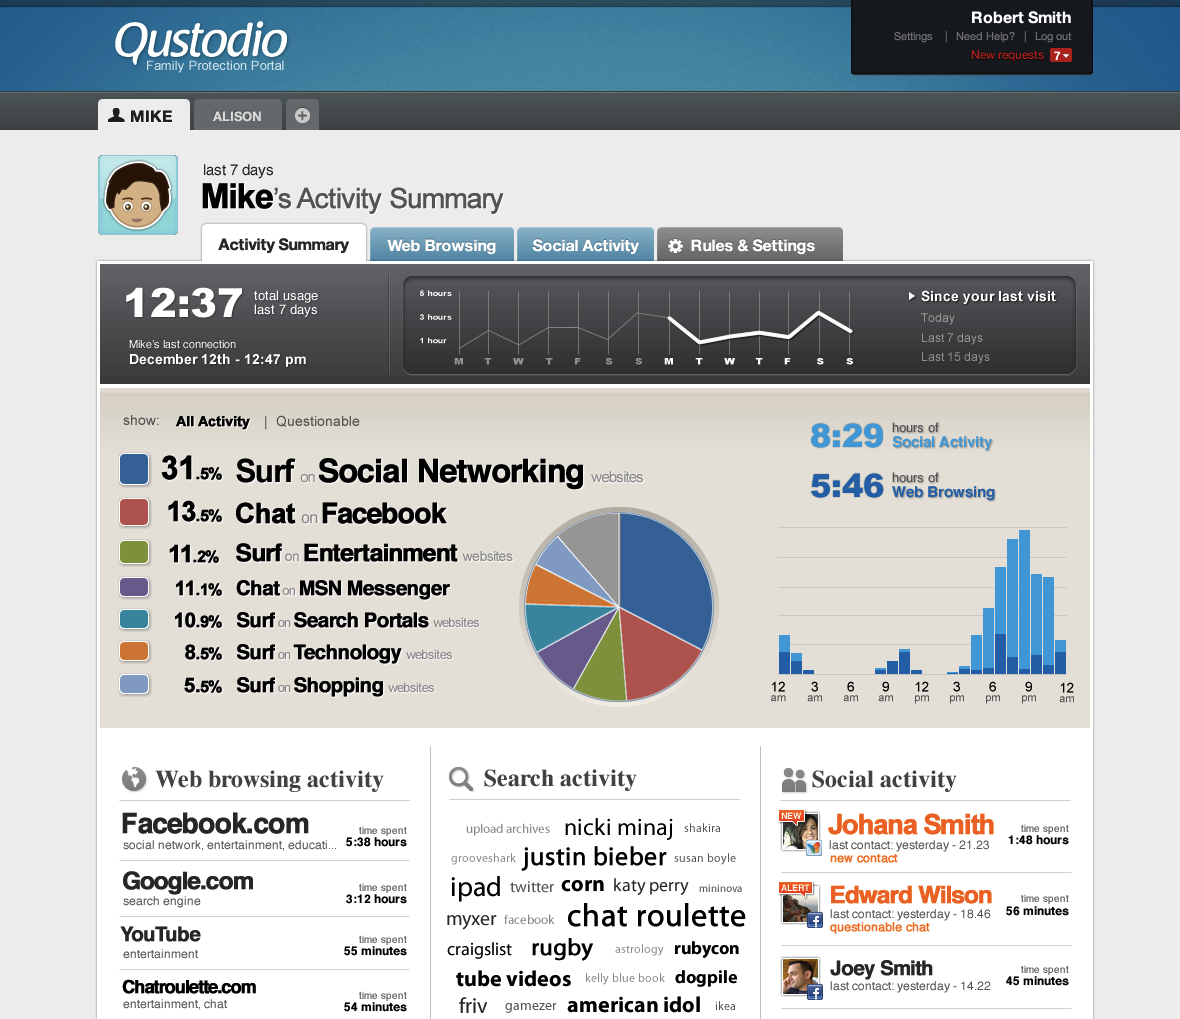
\includegraphics[width=1\textwidth]{Figures/qustodio}
\decoRule
\caption{Qustodio Reports}
\label{fig:qustodio}
\end{figure}

\subsection{Web Filtering}

The default configuration blocks all access for websites from ten undesirable categories, among them Drugs, Gambling, Pornography and Violence, and other 19 categories are available for more fine tuning. You can also configure an automatic notification when blocking a site. The content filtering is not dependent on the browser used and uses real-time analysis to supplement category database. It can also block HTTPS content, so it cannot be bypassed using an anonymizing proxy, but it does not have a feature to request temporary access for some blocked sites.

\subsection{Time Usage Limits}

You can control the usage by defining a weekly schedule in one-hour increments per device or by setting a daily maximum for each day. The time tracking is done cross device, so you can make sure that a child does not exceed its daily limits. The system can also block the device, not just control its internet access. Access to any mobile application can be blocked, with some limitations on iOS. Time limits can be controlled at the application level, so you can limit the amount of time the child spends on certain social media apps during the school week.

\subsection{Social Monitoring and Location Reporting}

Social media monitoring on Qustodio is limited to Facebook. You can see the child's Facebook wall activity on the online dashboard, including posts, pictures and comments, as well as the identity of any friends involved in online chats, but it does not report the content of those chats, to maintain some degree of privacy. It also includes location-reporting features, which you can use to check the child's location as often as every five minutes.

\subsection{Mobile Support}

The mobile application on Android offers features similar to the online portal. You can view all the children associated with the account and also set up another user profile, but you can't remove a child or change what device is associated with what profile. It redirects to the web portal when trying to make these changes. On the Android device, it can monitor all calls and SMS messages and you can choose to record the content of each message, block calls or restrict specific contacts, but this does not apply to third-party messaging apps like WhatsApp. Another feature specific to Android is the Panic Button, which works by configuring up to four trusted contacts which get notified in case of emergency. The iOS version cannot block or monitor calls and texts, because iOS blocks most interactions between applications, but the other features are almost identical to the Android version, with some more limitations related to location.\parencite{qustodioPCMag} We chose to not implement any call and SMS related features because we think that it goes beyond the scope of parental control, and that's why we do not implement any location related features.

\section{Circle with Disney}

Another system, which is more similar to ours, because it uses and external device connected to the local wireless network to implement parental control features is Circle with Disney. It is very easy configurable, because you only have to install it on the network and then use the simple mobile app to configure time limits and content filtering, among other features. The initial configuration is simple, you only have to plug the device in and connect to the device's hotspot, using the password supplied by the app to link the local Wi-Fi to Circle. The technology it uses is called ARP (Address Resolution Protocol) spoofing. The setup process is completed by configuring your own profile by choosing from five filter level: Pre-K, Kid, Teen, Adult and None. Next you have to identify the devices connected to the home network and choose a profile for them. You can leave some devices as unmanaged, and the others you can associated with the corresponding family member. You can add photos for each child user and you can associate the devices owned to the user profile, but the system assumes that a device is used by only one child, so you cannot control properly shared devices. \parencite{circlePCMag}

\subsection{ARP Spoofing}

The Address Resolution Protocol (ARP) is a communication protocol used for discovering the link layer address, such as a MAC address, associated with a given network layer address, typically an IPv4 address and provides a critical function in the Internet protocol suite. \parencite{plummer1982ethernet} It is a request-response protocol which sends messages encapsulated by a link layer protocol and only communicates within the boundaries of a single network, never routing across inter-networking nodes. This property places ARP into the link layer of the Internet protocol suite. \parencite{braden1989rfc} ARP Spoofing, also called ARP cache poisoning, is a technique generally used by an attacker to send (spoofed) Address Resolution Protocol (ARP) messages onto a local are network. The aim is to associate the attacker's MAC address with the IP address of another host, such as the default gateway, causing any traffic meant for that IP address to be sent to the attacker instead. It may allow the attacker to intercept data frames on the network, modify or stop all traffic, and is used to open other attacks, such as denial of service, man in the middle or session hijacking attacks. \parencite{ramachandran2005detecting} This kind of attack can be used only on networks that use ARP and requires the attacker to have access to the local network segment. \parencite{lockhart2004network}

\begin{figure}[th]
\centering
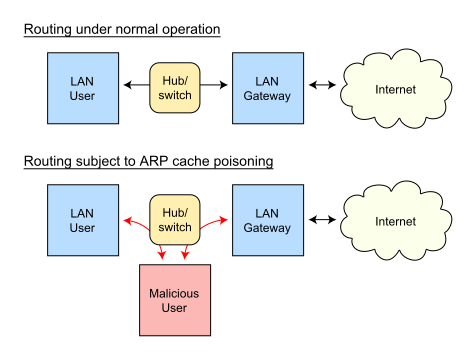
\includegraphics[width=1\textwidth]{Figures/arp-spoofing}
\decoRule
\caption{A successful ARP spoofing (poisoning) attack allows an attacker to alter routing on a network, effectively allowing for a man-in-the-middle attack}
\label{fig:circle}
\end{figure}

When sending and Internet Protocol Datagram from one host to another in a local network, the destination IP address must be resolved to a MAC address, so and ARP request packet is broadcasted, and the machine with the IP address from the request responds with an ARP reply that contains its MAC address. Since ARP is a stateless protocol, hosts will cache automatically the replies they receive and even ARP entries that have not expired yet will be overwritten when a new reply is received. The peer from which the packet originated have no method of authenticating with the host and this create the vulnerability that allows spoofing to occur. The techniques used in ARP spoofing are also used to implement redundancy of network services. Only two companies are known to date to have commercialized products centered around this strategy, and one of them is the parental control system, Disney Circle

\subsection{Blocking Platforms}

Each filter level comes with preconfigured platforms which you choose to block or unblock. Platforms refer to a list of Internet-aware apps. No platform is blocked at the Adult level, but for Teen level, HBO, Meerkat, Periscope, Reddit, Snapchat and Tumblr are blocked, for example, as we can see in the figure below. \parencite{circleMashable}

\begin{figure}[th]
\centering
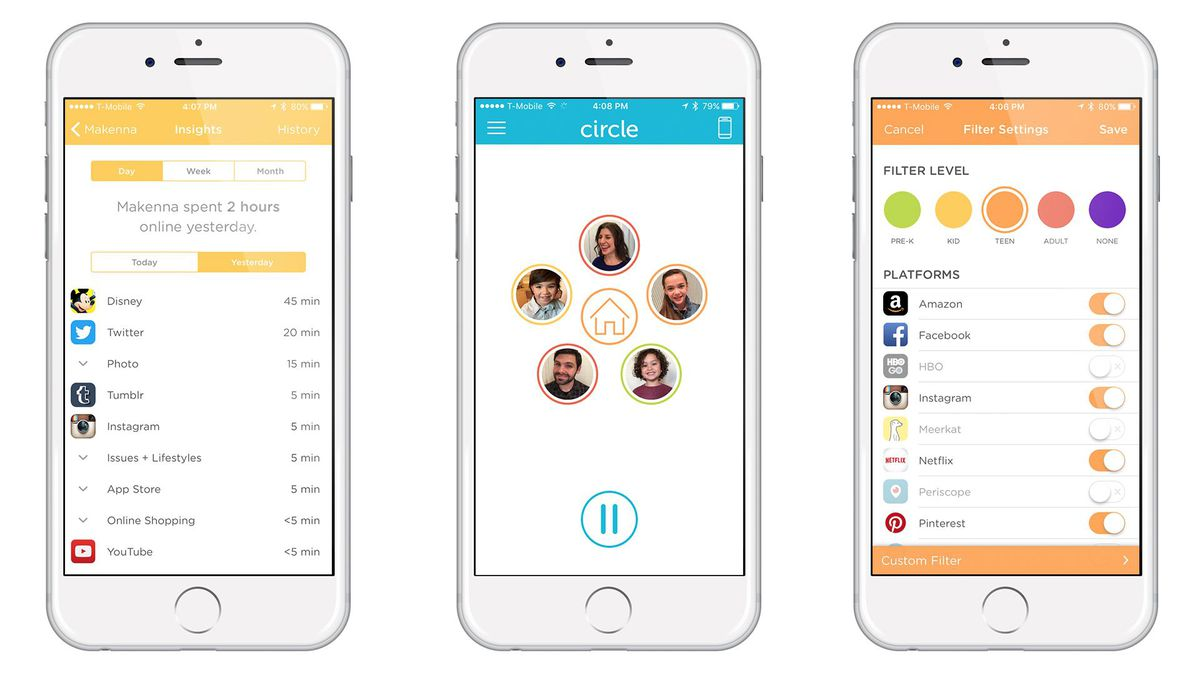
\includegraphics[width=1\textwidth]{Figures/circle}
\decoRule
\caption{Circle With Disney Main Features}
\label{fig:circle}
\end{figure}

\subsection{Content Filtering}

There are 30 content categories which can be allowed or blocked, depending on profile. Every profile have some categories blocked by default, even the Adult profile has Dating, Explicit Content, Gambling, Mature and VPN \& Proxies blocked. The Teen level blocks some more categories, while Kid level adds Social Media to the always-blocked list. For the Pre-K level, the only sites permitted are those from the Kids category. The changes to the filtering policies take effect immediately and since proxies are blocked by default, there is no way of getting around them. We chose to use the same approach and use an additional device on the network to implement the control policies, because it makes the experience device-independent.

\subsection{Privacy and Safety}

Circle offers also some privacy and safety settings, which are specific for each profile level. For example, Safe Search is forced in Google for Teen level, while the Kid level adds YouTube restrictions, and these restrictions are always on for Pre-K level.
There is even and ad blocking feature, which works fine, without breaking the page layouts. Even though ad blocking hurts the revenue of websites relying on advertising, we think that kids should not be involved in the advertising business, so we decided to include the ad blocking feature, by relying on the Pi-Hole system to block ads for children profile level.

\subsection{Time Limits, Bedtime and Pause}

Circle does not support weekly hour-by-hour Internet schedule the way other parental control systems do, but you can set a daily maximum for Internet access, which applies for all devices of a user. You can also set these daily limits for each platform or content categories. Internet access can be cut off for devices at a specified time, bed time, and will resume at the specified wakeup time. You cannot block access to any specific app, you can only cut the Internet access, since the device can control only the network. This can be a disadvantage, but is also more easy to configure such a system, because it may work without ever installing anything on the client device. Another feature that Circle offers is the pause function. You can choose to pause the internet access for all the managed devices, only for one child's devices or just for one specific device.

%----------------------------------------------------------------------------------------